% PHẦN TRÊN: LỀ TRÁI TRỐNG + CỘT CHÍNH CHỨA VÍ DỤ 6
\noindent
\begin{minipage}[t]{0.25\textwidth}
    \hfill
\end{minipage}%
\hfill
\begin{minipage}[t]{0.73\textwidth}
    \vspace{-4pt}
    \textbf{\textsf{\color{stewartcyan}VÍ DỤ 6}}\hspace{0.8em}Chứng minh đồng nhất thức $\tan^{-1}x + \cot^{-1}x = \pi/2$.\[3pt]
    \textbf{\textsf{\color{stewartcyan}LỜI GIẢI}}\hspace{0.8em}Mặc dù không nhất thiết phải dùng phép tính vi tích phân để chứng minh đồng nhất thức này, nhưng phép chứng minh dùng phép tính vi tích phân lại khá đơn giản. Nếu xét hàm số $f(x) = \tan^{-1}x + \cot^{-1}x$, thì
    \[
    f'(x) = \frac{1}{1 + x^2} - \frac{1}{1 + x^2} = 0
    \]
    với mọi giá trị của $x$. Do đó $f(x) = C$, một hằng số. Để xác định giá trị của $C$, ta chọn $x = 1$ [vì ta có thể tính chính xác giá trị $f(1)$]. Khi đó
    \[
    C = f(1) = \tan^{-1}1 + \cot^{-1}1 = \frac{\pi}{4} + \frac{\pi}{4} = \frac{\pi}{2}
    \]
    Vậy $\tan^{-1}x + \cot^{-1}x = \pi/2$.\hfill{\color{stewartcyan}\rule{1.1ex}{1.1ex}}
\end{minipage}

\vspace{8pt}

% THANH TIÊU ĐỀ PHÂN CÁCH BÀI TẬP (4.2 BÀI TẬP) VỚI 4 ĐƯỜNG KẺ CYAN CHUẨN NGUYÊN TÁC
\noindent
\begin{tikzpicture}[x=1pt, y=1pt]
    % 4 đường kẻ ngang bên trái
    \foreach \y in {4.5, 1.5, -1.5, -4.5} {
        \draw[stewartcyan, line width=0.55pt] (0, \y) -- (32, \y);
    }
    
    % Tiêu đề chính giữa
    \node[anchor=west, inner sep=0pt] (heading) at (38, 0) {
        {\sffamily\bfseries\color{stewartcyan}\LARGE 4.2}\hspace{9pt}%
        {\sffamily\bfseries\LARGE\color{stewartdarkgray}Bài tập}%
    };
    
    % 4 đường kẻ ngang bên phải kéo dài hết chiều rộng trang
    \foreach \y in {4.5, 1.5, -1.5, -4.5} {
        \draw[stewartcyan, line width=0.55pt] ([xshift=9pt]heading.east |- 0, \y) -- (\textwidth, \y);
    }
\end{tikzpicture}

\vspace{6pt}

% PHẦN BÀI TẬP CHIA THÀNH 2 CỘT CÂN BẰNG HOÀN TOÀN
\noindent
\begin{minipage}[t]{0.485\textwidth}
    % BÀI TẬP 1
    \textbf{1.}\hspace{0.4em}Cho đồ thị của hàm số $f$ như hình vẽ. Hãy kiểm tra xem $f$ có thỏa mãn các giả thiết của Định lý Rolle trên đoạn $[0, 8]$ hay không. Sau đó hãy ước lượng (các) giá trị của $c$ thỏa mãn kết luận của Định lý Rolle trên đoạn đó.
    
    \begin{center}
        \vspace{-3pt}
        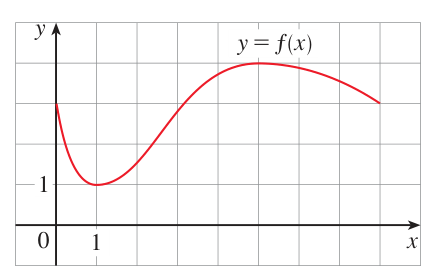
\includegraphics[width=0.68\linewidth]{images/p0330_fig1.png}
        \vspace{-3pt}
    \end{center}

    % BÀI TẬP 2
    \textbf{2.}\hspace{0.4em}Hãy vẽ đồ thị của một hàm số xác định trên $[0, 8]$ sao cho $f(0) = f(8) = 3$ và hàm số không thỏa mãn kết luận của Định lý Rolle trên đoạn $[0, 8]$.

    \vspace{4pt}
    % BÀI TẬP 3
    \textbf{3.}\hspace{0.4em}Cho đồ thị của hàm số $g$ như hình vẽ.
    
    \begin{center}
        \vspace{-3pt}
        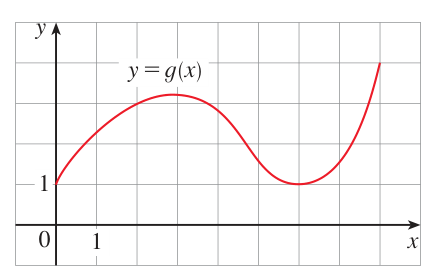
\includegraphics[width=0.68\linewidth]{images/p0330_fig2.png}
        \vspace{-3pt}
    \end{center}

    \begin{enumerate}[label=(\alph*), itemsep=1pt, topsep=1pt, parsep=0pt, leftmargin=1.5em]
        \item Kiểm tra xem $g$ có thỏa mãn các giả thiết của Định lý Giá trị Trung bình trên đoạn $[0, 8]$ hay không.
        \item Ước lượng (các) giá trị của $c$ thỏa mãn kết luận của Định lý Giá trị Trung bình trên đoạn $[0, 8]$.
        \item Ước lượng (các) giá trị của $c$ thỏa mãn kết luận của Định lý Giá trị Trung bình trên đoạn $[2, 6]$.
    \end{enumerate}

    \vspace{4pt}
    % BÀI TẬP 4
    \textbf{4.}\hspace{0.4em}Hãy vẽ đồ thị của một hàm số liên tục trên $[0, 8]$ thỏa mãn $f(0) = 1$ và $f(8) = 4$, đồng thời không thỏa mãn kết luận của Định lý Giá trị Trung bình trên đoạn $[0, 8]$.
\end{minipage}%
\hfill
\begin{minipage}[t]{0.485\textwidth}
    % NHÓM BÀI TẬP 5-8
    \textbf{\color{stewartcyan}5--8}\hspace{0.5em}Cho đồ thị của một hàm số $f$ như hình vẽ. Hàm số $f$ có thỏa mãn các giả thiết của Định lý Giá trị Trung bình trên đoạn $[0, 5]$ hay không? Nếu có, hãy tìm một giá trị $c$ thỏa mãn kết luận của Định lý Giá trị Trung bình trên đoạn đó.

    \begin{center}
        \vspace{-2pt}
        \setlength{\tabcolsep}{2pt}
        \begin{tabular}{cc}
            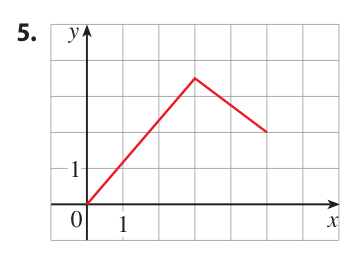
\includegraphics[width=0.47\linewidth]{images/p0330_fig3.png} &
            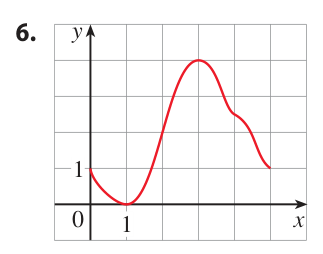
\includegraphics[width=0.47\linewidth]{images/p0330_fig4.png} \\[2pt]
            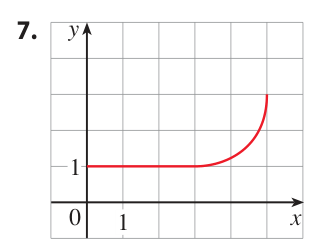
\includegraphics[width=0.47\linewidth]{images/p0330_fig5.png} &
            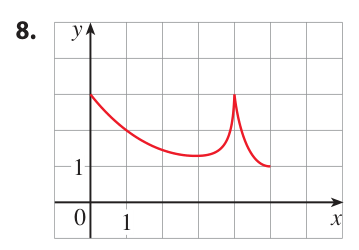
\includegraphics[width=0.47\linewidth]{images/p0330_fig6.png}
        \end{tabular}
        \vspace{-2pt}
    \end{center}

    {\color{stewartcyan}\hrule height 0.5pt}
    \vspace{4pt}

    % NHÓM BÀI TẬP 9-12
    \textbf{\color{stewartcyan}9--12}\hspace{0.5em}Kiểm tra xem hàm số có thỏa mãn ba giả thiết của Định lý Rolle trên đoạn đã cho hay không. Sau đó, tìm tất cả các số $c$ thỏa mãn kết luận của Định lý Rolle.

    \begin{enumerate}[label=\textbf{\arabic*.}, itemsep=1.5pt, topsep=1.5pt, parsep=0pt, leftmargin=1.8em]
        \setcounter{enumi}{8}
        \item $f(x) = 2x^2 - 4x + 5, \quad [-1, 3]$
        \item $f(x) = x^3 - 2x^2 - 4x + 2, \quad [-2, 2]$
        \item $f(x) = \sin(x/2), \quad [\pi/2, 3\pi/2]$
        \item $f(x) = x + 1/x, \quad \left[\frac{1}{2}, 2\right]$
    \end{enumerate}

    \vspace{3pt}
    {\color{stewartcyan}\hrule height 0.5pt}
    \vspace{4pt}

    % BÀI TẬP 13
    \textbf{13.}\hspace{0.4em}Cho hàm số $f(x) = 1 - x^{2/3}$. Chứng minh rằng $f(-1) = f(1)$ nhưng không tồn tại số $c$ nào trong khoảng $(-1, 1)$ sao cho $f'(c) = 0$. Tại sao điều này không mâu thuẫn với Định lý Rolle?

    \vspace{4pt}
    % BÀI TẬP 14
    \textbf{14.}\hspace{0.4em}Cho hàm số $f(x) = \tan x$. Chứng minh rằng $f(0) = f(\pi)$ nhưng không tồn tại số $c$ nào trong khoảng $(0, \pi)$ sao cho $f'(c) = 0$. Tại sao điều này không mâu thuẫn với Định lý Rolle?
\end{minipage}
